\documentclass[11pt,a4paper]{report}
\usepackage{geometry}
\usepackage{latexsym}
\usepackage{graphicx}
\usepackage{amsmath}
\usepackage[spanish]{babel}
\usepackage{multirow}
\usepackage{amssymb}
\usepackage{tikz}
\usepackage{subcaption}
\usepackage{natbib}

\newcommand*\circled[1]{\tikz[baseline=(char.base)]{
		\node[shape=circle,draw,inner sep=2pt] (char) {#1};}}
	

\setlength{\parindent}{0pt}

\date{}
\begin{document}
\title{Memoria Trabajo Lingüística Computacional}
\author{  Miguel This is a Placeholder\and Roberto Labadie Tamayo}
	\date{Octubre 2022}
	\maketitle
	
	
	\section*{Tarea I}
		
		Para evaluar la tarea de etiquetado morfosintágtico empleando un HMM entrenado sobre el corpus \textbf{cess-esp} se estudian dos variantes, una sobre una versión reducida del problema con un conjunto de categorías mas abarcadoras y la versión original usando las etiquetas tal cual aparecen en el corpus.
		\\
		A través de una validación cruzada con 10 particiones del dataset se obtienen los resultados como se muestran en la \figurename~\ref{HMM_task1}.
		
		\begin{figure}[!thb]
		\begin{center}
			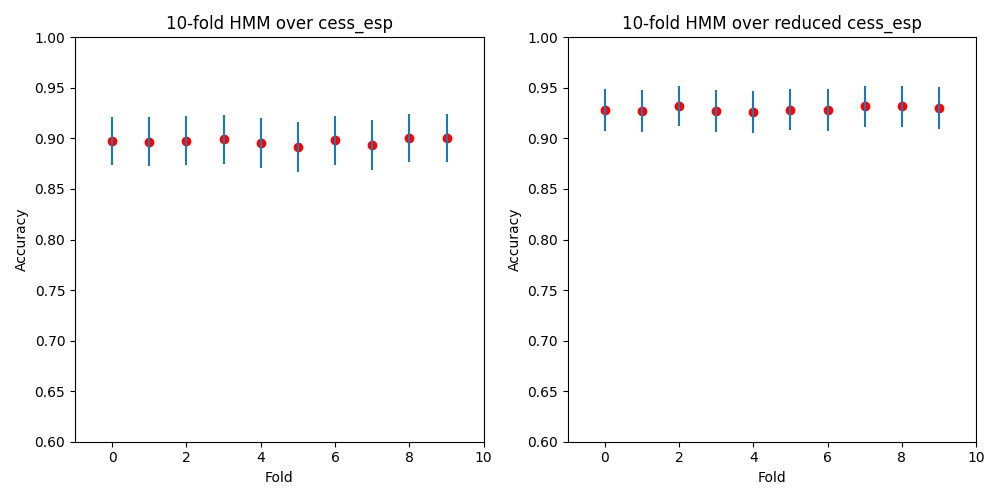
\includegraphics[scale=0.6]{images/HMM_task1.png}
		\end{center}
		\caption{Hidden Markov Model sobre cess-esp (izquierda) y cess-esp reducido (derecha) }
		\label{HMM_task1}
	\end{figure}
	
	Como se puede apreciar el desempeño del modelo es mejor para el dataset de la tarea reducida gracias a que la cantidad de estados ocultos del modelo es menor por tanto la posibilidad de escoger una transición errada disminuye, esta observación se puede realizar incluyendo además los intervalos de un  un 95\% de confianza estimados. Nótese ademas que en ambos modelos la $i-esima$ partición es exactamente la misma, i.e., el mismo conjunto de elementos ordenados en ambos modelos.
	
		\begin{table}[thb!]
		\begin{center} 		
			\begin{tabular}{cc} 
				\hline	
				\multirow{2}{*}{\textbf{cess-esp}}&\textbf{reduced}\\
				&\textbf{cess-esp}\\
				\hline
				0.897$\pm$0.02&0.928$\pm$0.02\\
				0.897$\pm$0.02&0.927$\pm$0.02\\
				0.898$\pm$0.02&0.932$\pm$0.02\\
				0.899$\pm$0.02&0.928$\pm$0.02\\
				0.896$\pm$0.02&0.927$\pm$0.02\\
				0.892$\pm$0.02&0.928$\pm$0.02\\
				0.898$\pm$0.02&0.928$\pm$0.02\\
				0.893$\pm$0.02&0.932$\pm$0.02\\
				0.900$\pm$0.02&0.932$\pm$0.02\\
				0.900$\pm$0.02&0.930$\pm$0.02\\
				\hline
			\end{tabular}
			\caption{Perplejidad sobre modelos de 3-gramas y 4-gramas}	
			\label{kk}
		\end{center}
	\end{table}		 	
	

	
	En la curva anterior se muestran los resultados para modelos de 1-gramas hasta 4-gramas sobre el test set, como es intuitivo modelos con construcciones más simples de elementos atómicos (gramas) tienden a presentar una distribución más suavizada y uniforme entre los elementos del vocabulario con respecto a construcciones más complejas (4-gramas y 5-gramas). De los modelos explorados el más robusto  resulto el de 4-gramas, con una preplejidad de $\sim$ 7.22.
	
		\section*{Tarea II}
		
		\noindent De los resultados anteriores, resulta congruente pensar que empleando modelos de 3-gramas o 4-gramas podrían arrojar los mejores resultados, explorando distintos métodos de descuento como se muestra en la \figurename~\ref{k} curva. 
	
		\begin{figure}[!thb]
			\begin{center}
				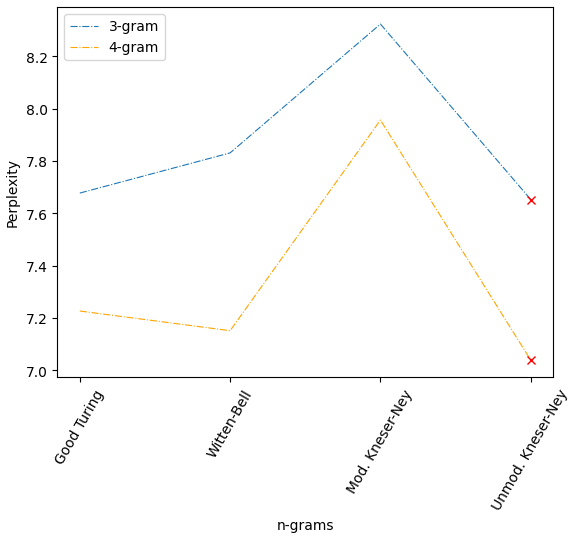
\includegraphics[width=280pt]{images/t2.png}
			\end{center}
			\caption{Resultados de Perplejidad sobre Dihana test set para modelos de 1-gramas a 4-gramas y distintos métodos de descuento .}
			\label{k}
		\end{figure}
		
	Nuevamente, para todos los casos los mejores resultados se obtienen para los modelos más complejos de 4-gramas, sin embargo el método no modificado de Kneser-Ney mejora los valores de perplejidad con respecto a las otras variantes de descuento hasta el valor de ~7.04 en 4-gramas y 7.65 para 3-gramas.
	
	\section*{Tarea III}
	
	\noindent Al sustituir el suavizado mediante back-off por un esquema de interpolación sobre los descuentos  de Witten-Bell y Kneser-Ney modificado, los resultados obtenidos en términos de perplejidad se muestran en el \tablename~\ref{kk}
	
	\begin{table}[thb!]
	\begin{center} 		
		\begin{tabular}{lcc|cc} 
			\hline	\multirow{2}{*}{Descuento}&\multicolumn{2}{c}{3-gram}&\multicolumn{2}{c}{4-gram}\\
			\cline{2-5}
			&\textit{Back-off}&\textit{Interpol.}&\textit{Back-off}&\textit{Interpol.}\\
			\hline
			Witten-Bell&7.83&\textbf{7.36}&7.15&\textbf{6.58}\\
			Kneser-Ney&8.32&\textbf{7.70}&7.96&\textbf{7.02}\\
			\hline
		\end{tabular}
		\caption{Perplejidad sobre modelos de 3-gramas y 4-gramas}	
		\label{kk}
	\end{center}
\end{table}		 	
	\noindent Donde como se puede observar en cada caso los valores son mejorados tanto para los modelos de 3-gramas como para 4-gramas, donde se obtienen los mejores resultados.
	
	\section*{Tarea IV}
	
	\noindent Para estudiar como impacta el uso de conjuntos léxicos con distintas cargas semánticas, se analiza el desempeño de modelos de 3-gramas y 4-gramas bajo las mismas condiciones de la tarea I, i.e., descuento de Good-Turing y suavizado de back-off empleando el conjunto de datos Europarl. Este estudio consiste simplemente en remover del vocabulario términos de forma escalonada que aparecen 1, 5 o menos y 9 o menos veces. 
	
	\begin{figure}[!thb]
		\begin{center}
			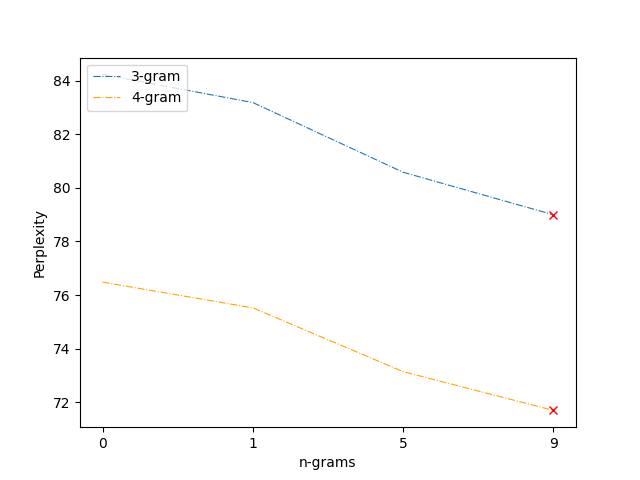
\includegraphics[width=300pt]{images/t4.png}
		\end{center}
		\caption{Resultados de Perplejidad sobre reducciones de vocabulario para dataset Europal en modelos de 3-gramas y 4-gramas.}
	\end{figure}

	\noindent Como se puede observar, modelos de 4-gramas poseen un mejor comportamiento en todas las variaciones. Para el valor de 0 (no eliminando palabra alguna del vocabulario) se obtienen los resultados más altos de perplejidad lo cual es coherente con el hecho de que elementos más uniformemente distribuidos poseen menor entropía y por tanto perplejidad. Esta condición de uniformidad se aproximará mientras nos acercamos al valor del 9 ya que se eliminan términos extremos. Por otro lado, términos menos frecuentes dentro de un corpus son en gran parte aquellos que caracterizan el lenguaje de manera específica y por tanto lo complejizan de ahí gran parte de este decrecimiento.
	
\end{document}